% Desenvolvido por: Prof. Dr. David Buzatto
% Modificado por: Brian Sena. 
% Versão 0.1
% Data: 01/08/2023
%\documentclass[notes, aspectratio=169]{beamer}
\documentclass[aspectratio=169]{beamer}
\usepackage{structure}
\usepackage{array}
\usepackage{graphicx}
\usepackage{makecell}
\renewcommand\theadalign{bc}
\renewcommand\theadfont{\bfseries}
\renewcommand\theadgape{\Gape[4pt]}
\renewcommand\cellgape{\Gape[4pt]}

\newcommand\blfootnote[1]{%
  \begingroup
  \renewcommand\thefootnote{}\footnote{#1}%
  \addtocounter{footnote}{-1}%
  \endgroup
}


\captionsetup{justification=centering}


%\usepackage[alf,abnt-emphasize=bf]{abntex2cite}
%\usepackage[backend=biber, defernumbers=true, style=numeric-comp, bibstyle=ieee, sorting=none]{biblatex}
\usepackage[style=verbose,maxnames=10,babel=hyphen,hyperref=true,abbreviate=true,backend=biber,mcite]{biblatex}
% Configurando BibLaTeX
\DefineBibliographyStrings{spanish}{
  url = {URL},
  andothers={et ~al\adddot}
}

\addbibresource{bibliografia/bibliografia.bib}

\setbeamercovered{transparent}

\setbeamertemplate{endpage}{%
  \subsection*{Dudas, preguntas o comentarios.}
  \begin{frame}[noframenumbering]
      \frametitle{Agradecimientos}
      \begin{center}
      \Huge Gracias por su atención.
      \par\bigskip
      \large ¿Dudas, preguntas o comentarios?
      \end{center}
    \end{frame}
}

\AtEndDocument{\usebeamertemplate{endpage}}
\begin{document}

\titulo{Estimación de la calidad de imágenes médicas 3D por
medio de aprendizaje automático}
\autor{Brian Sena Simons.}
\orientador{Dr. Pablo Mesejo Santiago.}
\coorientador{Dr. Enrique Bermejo Nievas.}
\github{\url{https://github.com/CodeBoy-source/TFG_NRPCQA}}

\title[TFG]{\titulo}
\author[Brian Sena Simons]{Brian Sena Simons}
\institute[UGR]{Universidad de Granada}
\date{\today}

\curso{Grado en Ingeniería Informática}

\local{Granada}

\chapter*{}
%\thispagestyle{empty}
%\cleardoublepage

%\thispagestyle{empty}

% \begin{titlepage}
 
\setlength{\centeroffset}{-0.5\oddsidemargin}
\addtolength{\centeroffset}{0.5\evensidemargin}

\thispagestyle{empty}

\noindent\hspace*{\centeroffset}\begin{minipage}{\textwidth}

\centering
%
\includegraphics[width=0.9\textwidth]{imagenes/logo_ugr.jpg}\\[0.4cm]

%\textsc{ \Large PROYECTO FIN DE CARRERA\\[0.2cm]}
%\textsc{ INGENIERÍA EN INFORMÁTICA}\\[1cm]
% Upper part of the page
% 

 \vspace{3.3cm}

%si el proyecto tiene logo poner aquí

\includegraphics{imagenes/logo.png} 
 \vspace{0.5cm}

% Title

{\Huge\bfseries \myTitle\\
}
\noindent\rule[-1ex]{\textwidth}{3pt}\\[3.5ex]
{\large\bfseries \mySubTitle\\[4cm]}
\end{minipage}

\vspace{2.5cm}
\noindent\hspace*{\centeroffset}\begin{minipage}{\textwidth}
\centering

\textbf{Autor}\\ {\myName}\\[2.5ex]
\textbf{Directores}\\
{\myProf\\
\myOtherProf}\\[2cm]
%
\includegraphics[width=0.15\textwidth]{imagenes/tstc.png}\\[0.1cm]
%\textsc{\myDepartment}\\
%\textsc{---}\\
%Granada, mes de 201
\end{minipage}
%\addtolength{\textwidth}{\centeroffset}
\vspace{\stretch{2}}

 
\end{titlepage}



%\cleardoublepage
%\thispagestyle{empty}

\pagestyle{fancyplain}
\begin{center}
{\large\bfseries \myTitle: \mySubTitle }\\
\end{center}
\begin{center}
\myName\\
\end{center}

%\vspace{0.7cm}
\noindent{\textbf{Palabras clave}: palabra\_clave1, palabra\_clave2, palabra\_clave3, ......}\\

\vspace{0.7cm}
\noindent{\textbf{Resumen}}\\

Poner aquí el resumen.
\cleardoublepage


% @TODO: Uncomment
%\thispagestyle{empty}


\begin{center}
{\large\bfseries \myTitle: \mySubTitle}\\
\end{center}
\begin{center}
\myName \\
\end{center}

%\vspace{0.7cm}
\noindent{\textbf{Keywords}: Keyword1, Keyword2, Keyword3, ....}\\

\vspace{0.7cm}
\noindent{\textbf{Abstract}}\\

Write here the abstract in English.

\chapter*{}
% @TODO: Uncomment
%\thispagestyle{empty}

\noindent\rule[-1ex]{\textwidth}{2pt}\\[4.5ex]

Yo, \textbf{\myName}, alumno de la titulación TITULACIÓN de la \textbf{\myFaculty}, 
con Pasaporte NX4L843F5, autorizo la ubicación de la siguiente copia de mi 
Trabajo Fin de Grado en la biblioteca del centro para que pueda ser
consultada por las personas que lo deseen.

\vspace{6cm}

\noindent Fdo: \myName

\vspace{2cm}

\begin{flushright}
Granada a X de mes de 201 .
\end{flushright}


\chapter*{}
% @TODO: Uncomment
%\thispagestyle{empty}

\noindent\rule[-1ex]{\textwidth}{2pt}\\[4.5ex]

D. \textbf{\myProf}, Profesor del Área de \todo[caption={Pendiente de completar: Área del tutor}]{No sé exactamente que poner aquí}XXXX del \myDepartment de la Universidad de Granada.

\vspace{0.5cm}

D. \textbf{\myOtherProf}, Profesor del Área de \todo[caption={Pendiente de completar: Área del co-tutor}]{No sé exactamente que poner aquí}XXXX del \myDepartment de la Universidad de Granada.


\vspace{0.5cm}

\textbf{Informan:}

\vspace{0.5cm}

Que el presente trabajo, titulado \textit{\textbf{\myTitle, \mySubTitle}},
ha sido realizado bajo su supervisión por \textbf{\myName}, y autorizamos la defensa de dicho trabajo ante el tribunal
que corresponda.

\vspace{0.5cm}

Y para que conste, expiden y firman el presente informe en Granada a X de mes de 201 .

\vspace{1cm}

\textbf{Los directores:}

\vspace{5cm}

\noindent \textbf{\myProf \ \ \ \ \ \myOtherProf}

\chapter*{Agradecimientos}
% @TODO: Uncomment

% \thispagestyle{empty}
       \vspace{1cm}


Poner aquí agradecimientos...

\section[Introducción]{Introducción}
\subsection[Contexto]{Contexto}
\begin{frame}
    \frametitle{Contexto}
    \begin{columns}
      \column{0.6\textwidth}
    \begin{enumerate}
      \item \textbf{La información visual} es cada vez más \textbf{importante}.
        \begin{itemize}
          \item Tanto para el entretenimiento como para el ámbito biomédico.
        \end{itemize}
      \item{Tarea de medir y cuantificar} la calidad perceptual humana de una imagen (IQA). 
        \begin{itemize}
          \item Factores importantes: \textbf{contenido, contraste, distorsiones y la percepción humana}
        \end{itemize}
    \end{enumerate}
    \column{0.4\textwidth}
    \begin{figure}
      \begin{center}
        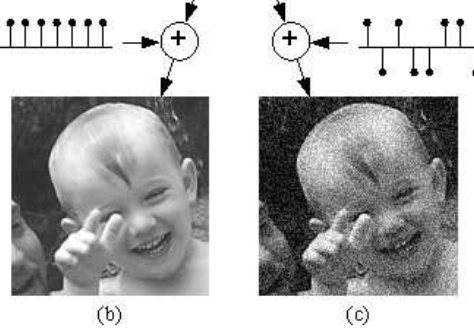
\includegraphics[width=\textwidth]{imagenes/chapter1/failure_minkowski_metricBIG}
      \end{center}
      \caption{Imágenes distorsionadas equidistantes\footnotemark}
    \end{figure}
  \end{columns}
  \vspace{-.2cm}
  \footcitetext{MinkowskiFailure}
\end{frame}

\begin{frame}
  \frametitle{Subproblemas}
  \vspace{-.5cm}
  \begin{figure}
    \caption{Figuras (a) y (b): problemas con referencia (FR) y sin referencia (NR).}
    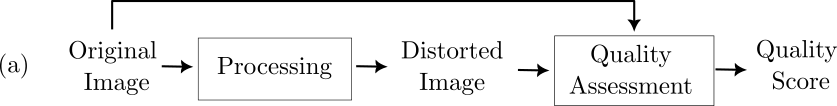
\includegraphics[width=0.8\textwidth]{imagenes/chapter1/HFullReferenceInk.png}
  \end{figure}
  \begin{figure}
    
\includegraphics[width=0.8\textwidth]{imagenes/chapter1/NoReferenceInk.png}
  \end{figure}
  \begin{enumerate}
    \item (b) es el subproblema más \textbf{difícil}.
    \item Debemos disponer de conocimientos generales sobre: 
      \begin{enumerate}
        \item Naturaleza de las imágenes.
        \item Efecto de las distorsiones.
      \end{enumerate}
  \end{enumerate}
\end{frame}


\subsection{Motivación}
\begin{frame}
  \frametitle{Aplicaciones}
  \begin{columns}
    \column{0.5\textwidth}
  \begin{enumerate}
      \item\textbf{Comparativa} entre algoritmos de compresión.
      \item\textbf{Recuperación} de la información.
      \item\textbf{Evaluar} errores de transmisión.
  \end{enumerate}
  \column{0.5\textwidth}
  \begin{figure}
    \begin{center}
      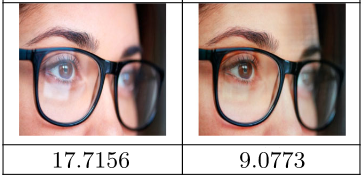
\includegraphics[width=0.85\textwidth]{imagenes/chapter1/Brisque}
    \end{center}
    \caption{
      Eliminación de reflejos en imágenes\footnote[frame]{\cite{BRISQUEExample}}
      con medida de calidad BRISQUE\footnote[frame]{\cite{BRISQUE}} (menor es mejor).
  }
  \end{figure}
  \end{columns}
\end{frame}

\begin{frame}
  \frametitle{Motivación}
  \begin{columns}
    \column{0.5\textwidth}
    \begin{enumerate}
    \item Cada vez \textbf{más frecuentemente} se emplean volúmenes tridimensionales.
    \item Las contribuciones relativas al IQA en la medicina resulta en: 
      \begin{itemize}
        \item \textbf{Reducción de costes}. 
        \item Reducción de tiempo de consulta.
        \item \textbf{Mejora de calidad del diagnóstico}.
      \end{itemize}
    \item La naturaleza de las imaǵenes médicas \textbf{reduce} la precisión de modelos IQA estándares.
    \end{enumerate}
  \column{0.5\textwidth}
  \begin{figure}
    \begin{center}
      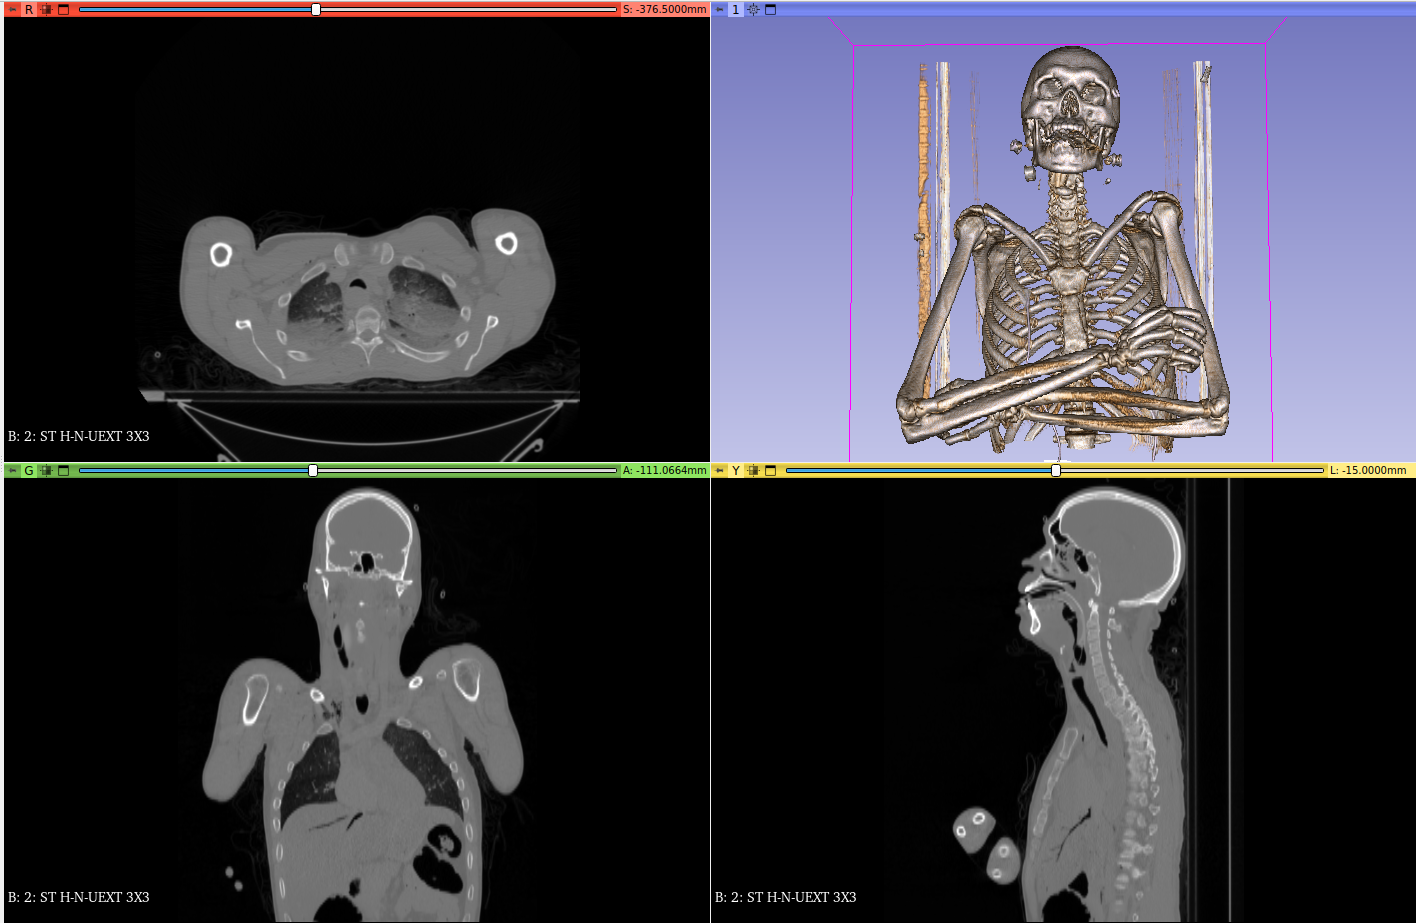
\includegraphics[width=0.95\textwidth]{imagenes/chapter1/SlicerVisualization}
    \end{center}
    \caption{Ejemplo de visualización 3D (Slicer\footnotemark).}
  \end{figure}
  \end{columns}
  \footcitetext{Slicer3D}
\end{frame}


\begin{frame}
  \frametitle{Motivación}
  \vspace{-0.2cm}
  \begin{columns}
    \column{0.5\textwidth}
  \begin{enumerate}
    \item As veces no tenemos acceso a las imágenes médicas 2D.
    \item Las distorsiones sobre dichas imágenes \textbf{afectan al volumen 3D generado}. 
    \item Dichas reconstrucciones suelen ser en forma de nubes de puntos.
    \item El número de métodos propuestos para 3D \textbf{decrece sustancialmente}.
  \end{enumerate}
  \column{0.5\textwidth}
  \begin{figure}
    \begin{center}
      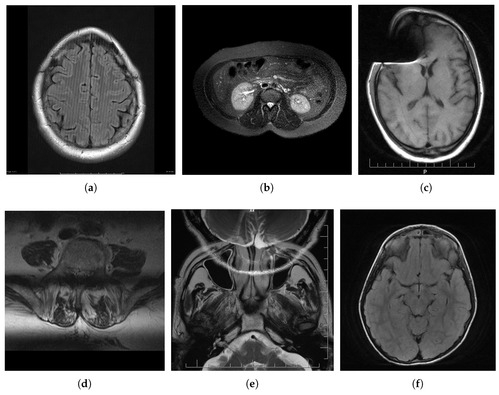
\includegraphics[width=0.78\textwidth]{imagenes/chapter1/MedicalDistortions}
    \end{center}
    \caption{Ejemplo de distorsiones médicas\footnotemark.}
  \end{figure}
  \end{columns}
  \footcitetext{MoreMedicalDistortion}
\end{frame}

\subsection{Objetivos}
\begin{frame}
  \frametitle{Objetivos}
  \begin{columns}

    \column{0.3\textwidth}
    \vspace{-1cm}
  \begin{enumerate}
    \item Estudio exhaustivo del estado del arte. 
    \item Generación de datos sintéticos.
    \item Validar métodos más prometedores.
  \end{enumerate}

  \column{0.7\textwidth}
  \vspace{-.2cm}
  \begin{figure}
      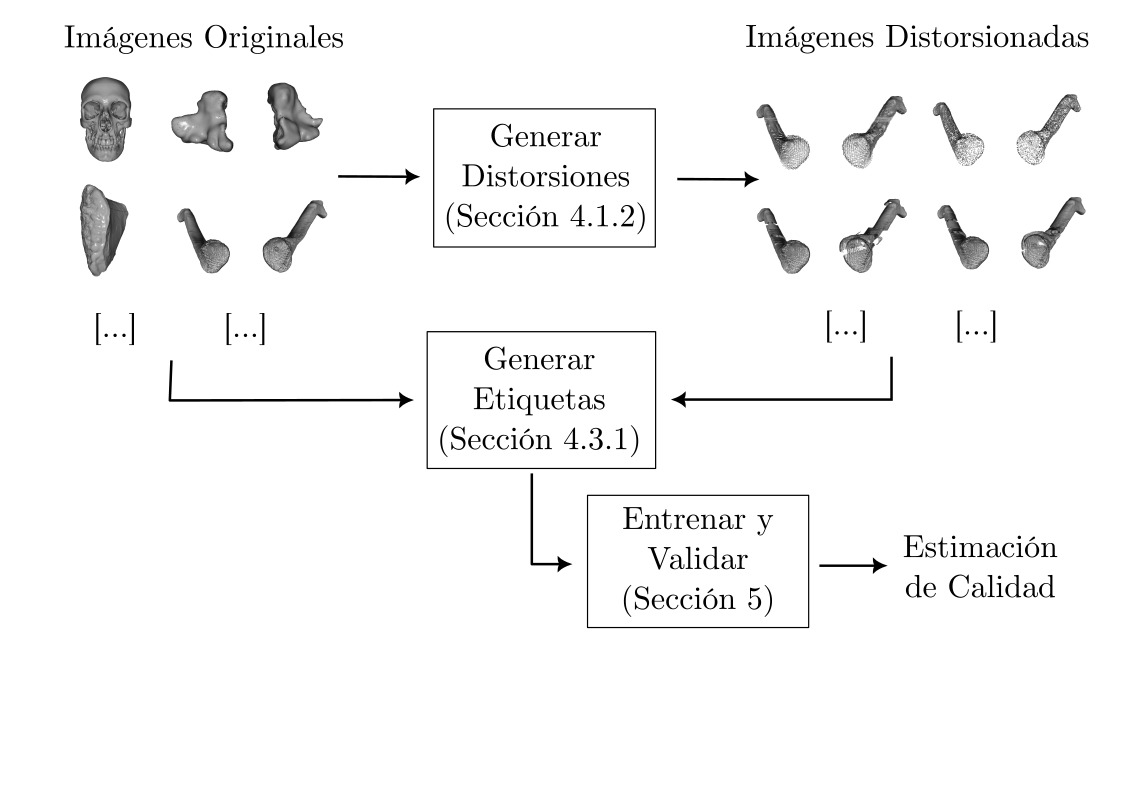
\includegraphics[width=1.0\textwidth, left]{imagenes/chapter1/Objetivos}
  \end{figure}

  \end{columns}
\end{frame}

\section{Estado del arte}
\subsection{Búsquedas Scopus}
\begin{frame}
    \frametitle{Tendencia Scopus}
    \begin{columns}
      \column{0.5\textwidth}
      \begin{figure}
        \begin{center}
          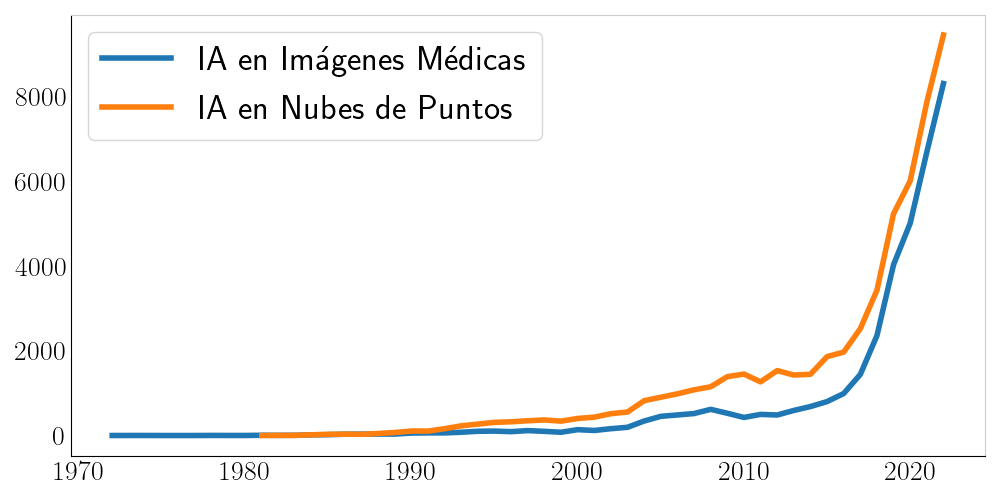
\includegraphics[width=\textwidth]{imagenes/chapter2/ScopusMLinMedicineAndPC}
        \end{center}
        \caption{Aprendizaje automático en medicina (azul) y nubes de puntos (naranja).
        \textbf{Ambos superan los 6000 documentos}.}
      \end{figure}
      
      \column{0.5\textwidth}
      \begin{figure}
        \begin{center}
          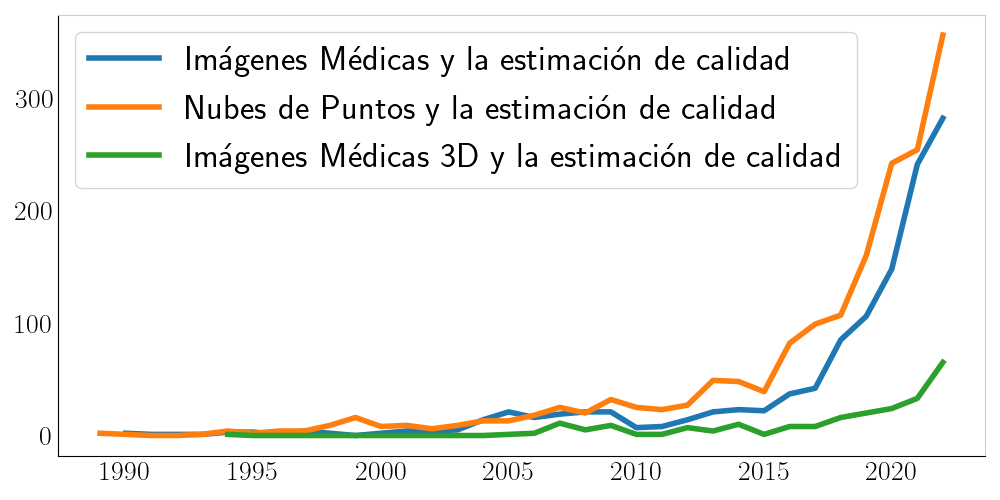
\includegraphics[width=\textwidth]{imagenes/chapter2/ScopusQualityAssessment}
        \end{center}
        \caption{Estimación de calidad en imágenes médicas (azul), nubes de puntos (naranja) 
          y en imágenes médicas 3D (verde). Esta última, tan solo llega a \textbf{60 publicaciones}}
      \end{figure}
    \end{columns}
\end{frame}

\subsection{Estado del arte IQA: métricas}
\begin{frame}
  \frametitle{Estado del arte IQA: métricas}
  \begin{columns}
    \column{0.5\textwidth}
    \begin{enumerate}
      \item Están basados en los avances del conocimiento sobre el sistema visual humano (HVS):
        \begin{enumerate}
          \item Cuantificación de la señal. 
          \item La \textbf{sensibilidad al contraste}.
          \item Hipótesis de percepción a través de: \textbf{brillo, contraste y estructuras}.
          \item La \textbf{saliencia visual}. 
          \item Empleo de \textbf{modelos DL}.
        \end{enumerate}
    \end{enumerate}

    \column{0.5\textwidth}
  \begin{table}[htp]
    \footnotesize
    \centering
    \begin{tabular}{|c|c|c|c|}
      \hline
      \rowcolor[HTML]{FFC702}
      \cellcolor[HTML]{FFC702} &  \multicolumn{3}{c|}{\cellcolor[HTML]{FFC702}\textbf{LIVE}}\\ \cline{2-4}
      \rowcolor[HTML]{FFC702}
      \multirow{-2}{*}{\textbf{Métrica}} & SRCC & PLCC & RMSE \\ 
      \hline
                    \textbf<2>{PSNRHVS} & 0.919 & 0.903 & 12.540 \\
                    \hline
                     UQI & 0.894 & 0.899 & 11.982 \\
                    \hline
                     \textbf<3>{SSIM} & 0.948 & 0.845 & 8.946 \\
                    \hline
                     \textbf<4>{VSI} & 0.952 & 0.948 & 8.682 \\
                    \hline
                     DSS & 0.962 & 0.931 & 9.961 \\
                    \hline
                     \textbf<5>{CD-MMF} & \textbf{0.981} & \textbf{0.980} & \textbf{5.413}\\ 
                    \hline 
    \end{tabular}
    \caption[Progreso de las métricas FR.]{
      Progreso de las métricas FR conforme avanza los conocimientos del HVS, ML y DL\footnotemark.
      }
      \label{tab:SOTAFRIQA}
  \end{table}
  \end{columns}
\footcitetext{SurveyOf2D3DMetrics}
\end{frame}

\subsection{Estado del arte PCQA: métodos}
\begin{frame}
  \frametitle{Estado del arte PCQA: métodos}
  \begin{columns}
    \column{0.5\textwidth}
    \begin{enumerate}
      \item Métodos para casos específicos. 
      \item Extracción de características del vecindario del punto.
        \begin{enumerate}
          \item Características \textbf{geométricas}.
          \item Características \textbf{lumínicas}.
        \end{enumerate}
      \item Métodos genéricos por ML. 
      \item Métodos genéricos por DL.
        \begin{enumerate}
          \item \textbf{Proyecciones 2D.}
          \item \textbf{Interpretación 3D directa.}
          \item Mixto.
        \end{enumerate}
    \end{enumerate}

    \column{0.5\textwidth}
      \begin{table}[htp]
          \footnotesize
          \centering
          \begin{tabular}{|c|c|c|c|c|}
              \hline
              \rowcolor[HTML]{FFC702}
              \cellcolor[HTML]{FFC702} & \multicolumn{2}{c|}{\cellcolor[HTML]{FFC702}\textbf{STJU-PCQA}} & \multicolumn{2}{c|}{\cellcolor[HTML]{FFC702}\textbf{WPC}} \\ 
              \cline{2-5}
             \multirow{-2}{*}{\cellcolor[HTML]{FFC702}\textbf{MODELO}}  &\multicolumn{1}{c|}{\cellcolor[HTML]{FFC702} PLCC} & \multicolumn{1}{c|}{\cellcolor[HTML]{FFC702}SRCC} & \multicolumn{1}{c|}{\cellcolor[HTML]{FFC702}PLCC} & \multicolumn{1}{c|}{\cellcolor[HTML]{FFC702}SRCC} \\
              \hline
              IT-PCQA & 0.58 & 0.63 & 0.55  & 0.54\\
              \hline
              \textbf<2->{NR3DQA} & 0.738 & 0.714 & 0.651 & 0.647\\
              \hline
              GPA-Net & 0.806 & 0.78 & - & - \\
              \hline
              ResSCNN & 0.86 & 0.81 & 0.72 & 0.75\\
              \hline
              \textbf<3->{VQA-PC} & 0.863 & 0.85 & 0.797 & 0.796\\
              \hline
              MM-PCQA & \textbf{0.92} & \textbf{0.91} & \textbf{0.83} & \textbf{0.83}\\
              \hline
          \end{tabular}
          \caption[Estado del arte de modelos NR-PCQA]{
          Resumen del estado del arte de modelos NR-PCQA en dos datasets SJTU y WPC.
        }
      \end{table}
  \end{columns}
\end{frame}

\subsection{Estado del arte en imágenes médicas}
\begin{frame}
  \frametitle{Estado del arte en imágenes médicas}
  \vspace{-0.4cm}
  \begin{columns}
    \column{0.5\textwidth}
  \begin{enumerate}
    \item \textbf{No existe} una imagen o representación \textbf{``sin distorsión''} en la medicina.
    \item Los métodos \textbf{actuales} utilizan adaptaciones \textbf{IQA} para 
      exámenes médicos específicos como \textbf{MRI}.
    \item \textbf{No se ha encontrado} nada específico en la literatura sobre 
      métodos aplicados \textbf{directamente a reconstrucciones 3D}.
  \end{enumerate}
    \column{0.5\textwidth}
    \begin{figure}
      \begin{center}
        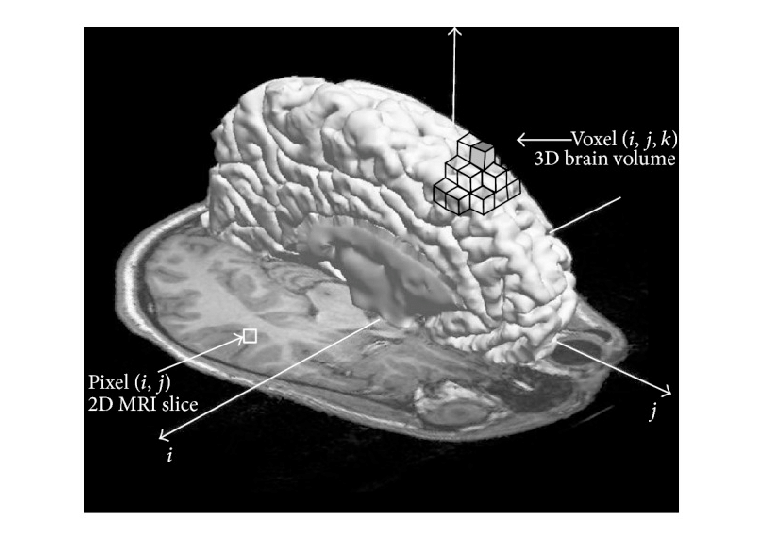
\includegraphics[width=0.95\textwidth]{imagenes/chapter2/MRIVoxel}
      \end{center}
      \caption{Generación de imagen volumétrica.}
      \label{fig:}
    \end{figure}
    
  \end{columns}
  \footcitetext{MRIVoxel}
\end{frame}

\section{Materiales y métodos}

\subsection{Materiales: datos generalistas}
\begin{frame}
    \frametitle{Materiales: datos generalistas (SJTU)}
    \begin{columns}
      \column{0.5\textwidth}
      \begin{enumerate}
        \item \textbf{10 nubes de puntos} de referencia.  
        \item \textbf{7} tipos de \textbf{distorsiones}: compresión, ruido al color, 
          ruido geométrico, ruido gaussiano y combinación entre ellas.
        \item \textbf{6 niveles} de intensidad.
        \item \textbf{Total de 420 nubes de puntos}.
      \end{enumerate}
      \column{0.5\textwidth}
      \begin{figure}
        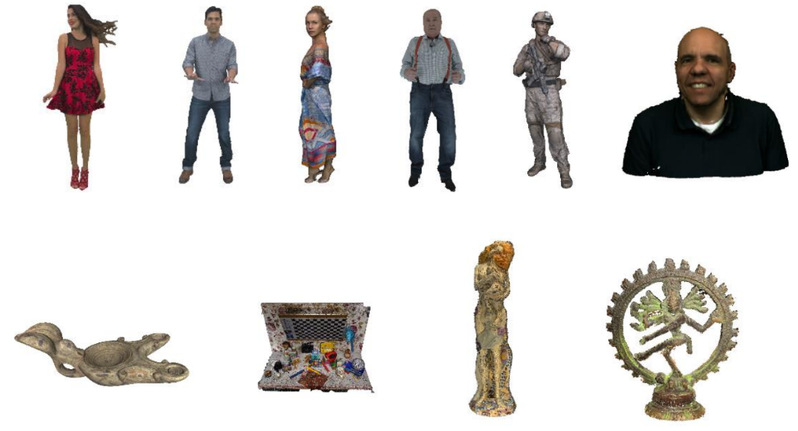
\includegraphics[width=0.95\textwidth]{imagenes/chapter3/SJTU}
        \caption{Ejemplo de conjuntos de datos SJTU\footnotemark}
        \label{fig:SJTU}
      \end{figure}
    \end{columns}
    \footcitetext{SJTU}
\end{frame}

\note{
Para el desarrollo de este proyecto, hemos hecho uso de diversos conjuntos de datos: 
El primero de ellos parte de 10 nubes de puntos 
a las cuales se aplican 7 tipos de distorsiones en 6 niveles de intensidad distintos. 
Luego, se obtiene una opinión media o MOS por sus siglas en inglés 
de 10 individuos para las 420 nubes de puntos. 
Dicho MOS sirve como medida de calidad de las mismas y para evaluar las 
predicciones del modelo. Es el procedimiento habitual.

}

\begin{frame}
    \frametitle{Materiales: datos generalistas (WPC)}
    \begin{columns}
      \column{0.5\textwidth}
      \begin{enumerate}
        \item \textbf{25 nubes de puntos} de referencia.  
        \item \textbf{5} tipos de \textbf{distorsiones}: 
          sumuestreo, ruido gaussiano, \emph{trisoup}, V-PCC y \emph{octree}.
        \item Longitud de \textbf{intensidades variantes}.
        \item \textbf{Total de 741 nubes de puntos}.
      \end{enumerate}
      \column{0.5\textwidth}
      \begin{figure}
        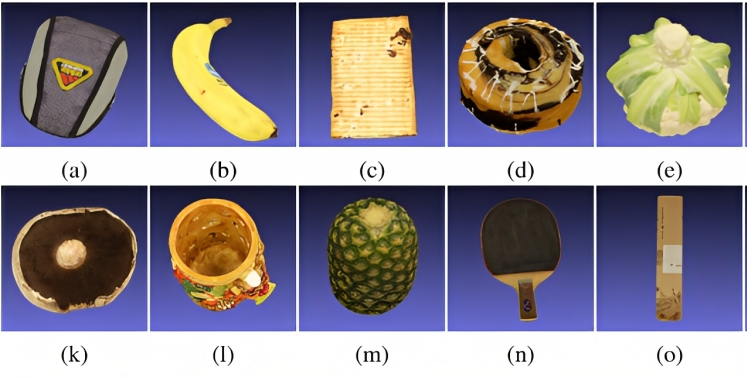
\includegraphics[width=.95\textwidth]{imagenes/chapter3/WPC}
        \caption{Ejemplo de conjuntos de datos WPC\footnotemark}
        \label{fig:WPC}
      \end{figure}
    \end{columns}
    \footcitetext{WPC1}
\end{frame}

\note{
A continuación uno similar: WPC, pero en este caso tenemos más nubes de puntos 
de partida y, mayoritariamente, distorsiones de compresión. Los niveles de 
distorsión dependen del tipo de compresión. En total tendremos 741 nubes de puntos. 
}

\begin{frame}
  \frametitle{Materiales: datos generalistas (LS-PCQA)}
  \begin{columns}
    \column{0.5\textwidth}
    \begin{enumerate}
      \item \textbf{104 nubes de puntos} de referencia.  
      \item \textbf{31} tipos de \textbf{distorsiones}.
      \item \textbf{7 niveles} de intensidad.
      \item \textbf{Total de 22000 nubes de puntos}.
    \end{enumerate}
    \column{0.5\textwidth}
    \begin{figure}
      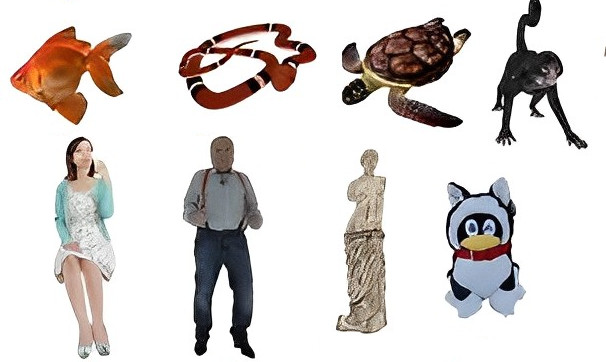
\includegraphics[width=0.8\textwidth]{imagenes/chapter3/LSPCQA}
      \caption{Ejemplo de conjuntos de datos LS-PCQA\footnotemark}
      \label{fig:LSSJTU}
    \end{figure}
  \end{columns}
  \footcitetext{ResSCNN}
\end{frame}

\note{
Luego, tenemos el reciente conjunto de datos sintético publicado en 2022.
Dicho conjunto de datos es considerado el mayor hasta la fecha, llegando a un 
total de 22000 nubes de puntos con 31 tipos de distorsiones distintas a 7 niveles 
de intensidad. 
}

\subsection{Materiales: datos sintéticos}
\begin{frame}
  \frametitle{Materiales: datos sintéticos}
  \vspace{-.8cm}
    \begin{figure}[htp]
      \subfloat[]{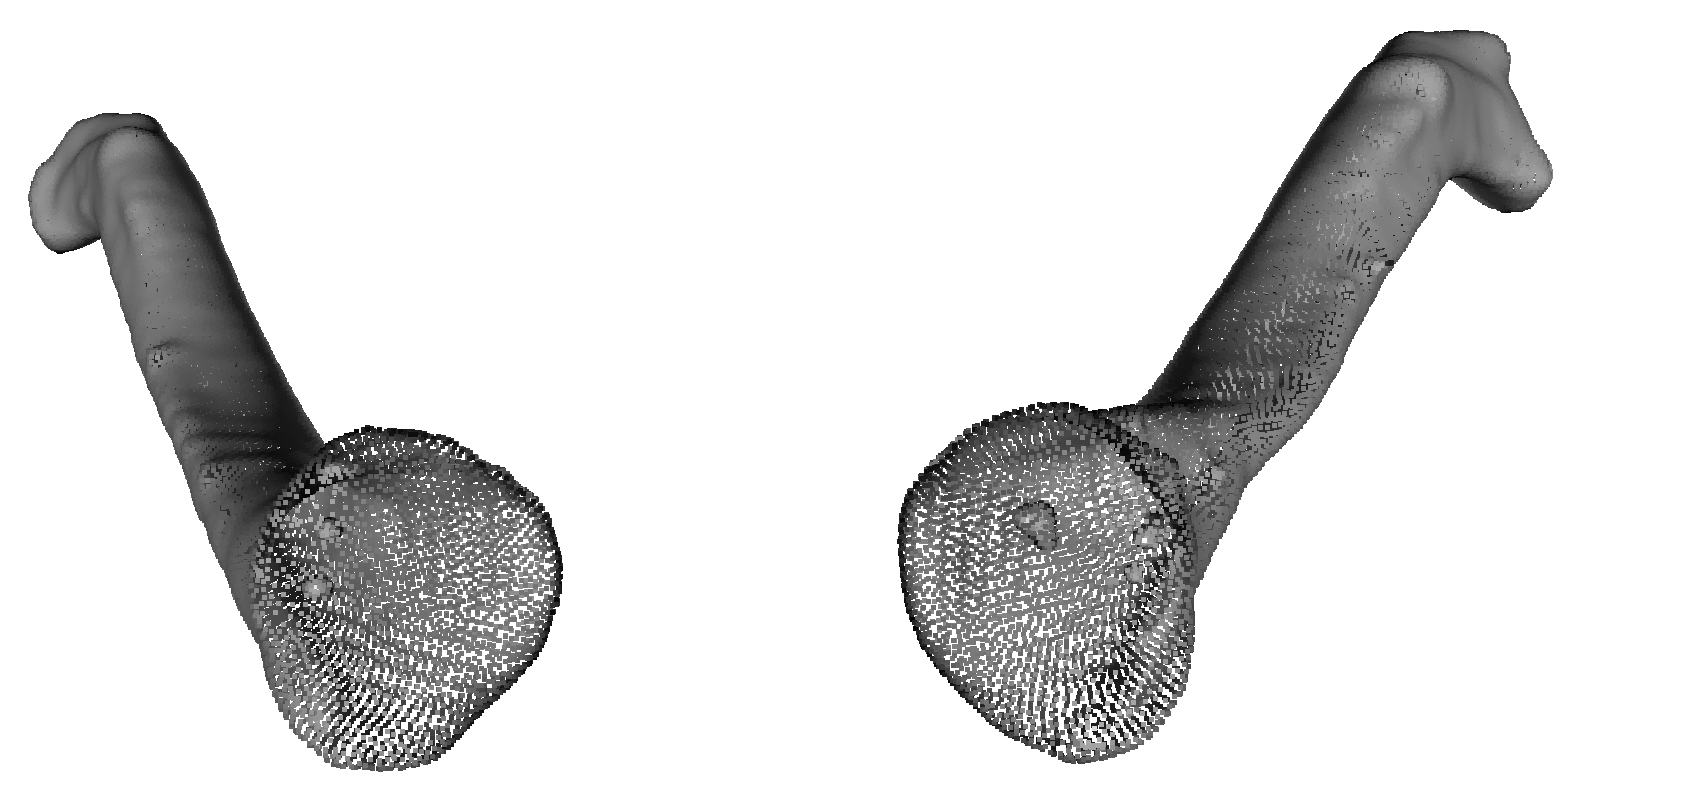
\includegraphics[width=.3\textwidth]{imagenes/chapter3/clavicula/clavicula_0.png}}
      \subfloat[]{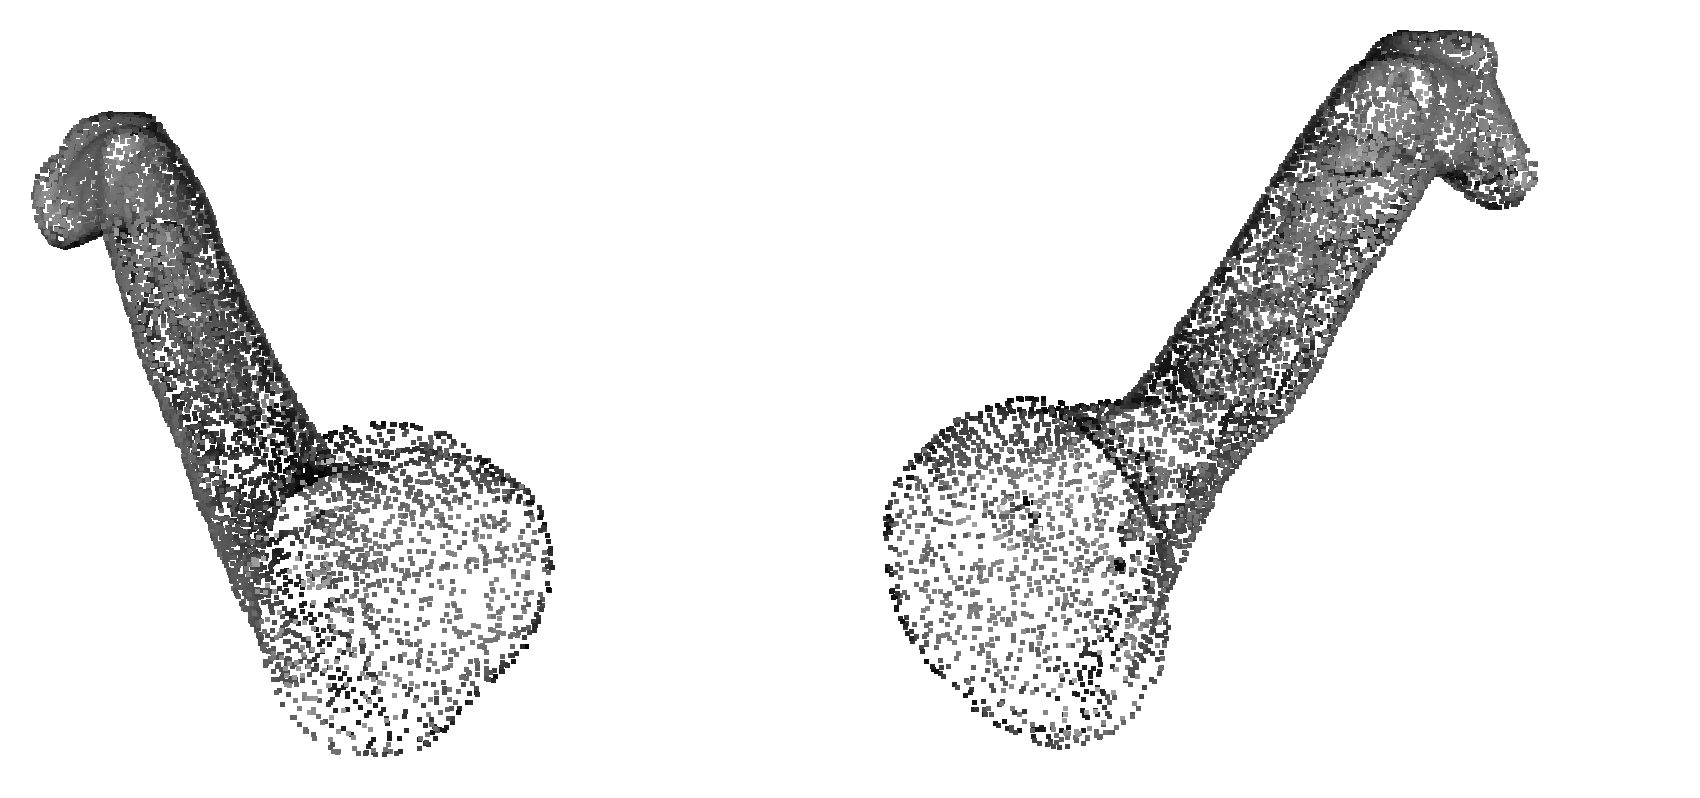
\includegraphics[width=.3\textwidth]{imagenes/chapter3/clavicula/clavicula_2.png}}
      \subfloat[]{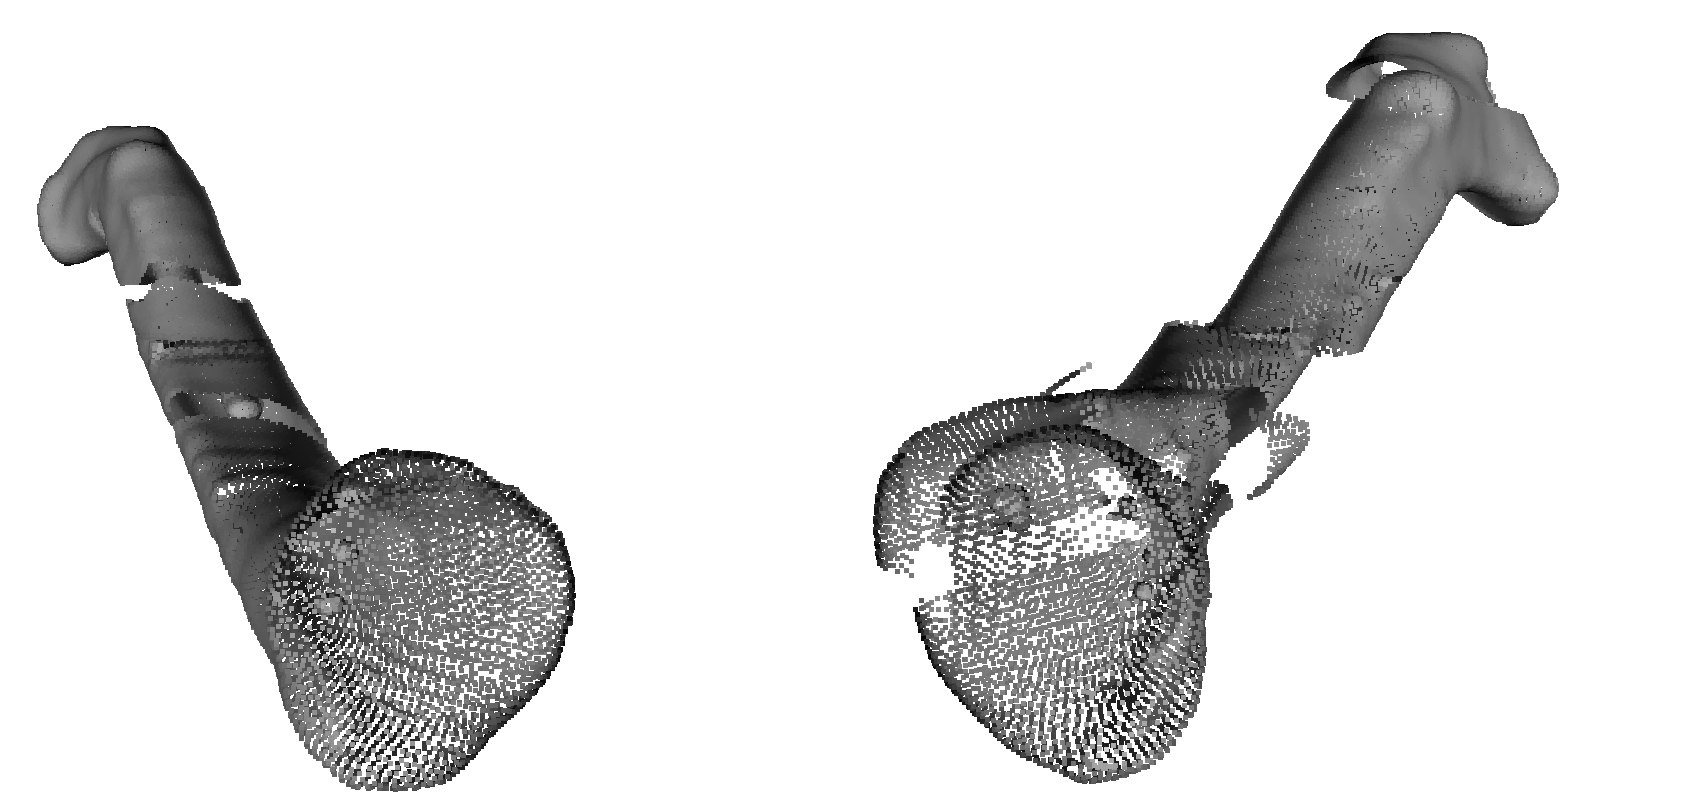
\includegraphics[width=.3\textwidth]{imagenes/chapter3/clavicula/clavicula_3.png}}
      \caption{Ejemplo de distorsiones generadas sobre clavículas, donde (a) es la imagen original, 
      (b) la distorsionada por submuestreo y (c) por movimiento local.}
      \label{fig:DistorsionesGeneradas}
    \end{figure}
  \vspace{-.3cm}
    \begin{enumerate}
      \item \textbf{11 nubes de puntos} de referencia.  
      \item \textbf{5} tipos de \textbf{distorsiones}: 
        submuestreo, compresión, ruido, rotación y movimiento local.
      \item \textbf{7 niveles} de intensidad para un \textbf{total de 385 nubes de puntos}.
    \end{enumerate}
\end{frame}

\note{
Por último, 
para la validación sobre un conjunto de datos médicos fue necesaria la creación 
de un conjunto de datos sintético. La razón es que 
no existe un conjunto de datos públicos para este análisis. 
Para ello estudiamos y fabricamos las 
distorsiones más comunes del ámbito biomédico con respecto a las reconstrucciones 3D. 
Disponemos de 11 nubes de puntos originales, 
sobre las cuáles se simulan 5 tipos de distorsiones 
a 7 niveles de intensidad cada una. Para un total de 385 representaciones.
En las distorsiones se simula tanto errores de transmisión, 
compresión, como el movimiento del paciente.
}

\begin{frame}
  \frametitle{Materiales: Generación de etiquetas}
  \begin{enumerate}
    \item Evitamos el problema logístico de obtención de la opinión media de calidad (MOS).
      \begin{itemize}
        \item Evaluación manual por grupo de personas en un entorno controlado.
      \end{itemize}
    \item Hacemos uso de las mejores métricas con referencia.
      \begin{itemize}
        \item Desglosamos el rendimiento por tipo de distorsión.
      \end{itemize}
  \end{enumerate}
\begin{table}
  \centering 
  \scriptsize
  \begin{tabular}{|c|c|c|}
    \hline
    \rowcolor[HTML]{FFC702}
     & \textbf{Parte I} & \textbf{Parte II} \\
    \hline 
    SROCC & 0.902697 & 0.878517\\
    \hline
    PLCC & 0.910713 & 0.871917\\
    \hline
  \end{tabular}
  \caption[Correlación de métricas sintéticas.]{
    Correlación de métricas sintéticas con experimento subjetivo de Liu et al\footnotemark[8].
}
  \label{tab:PseudoCorr}
\end{table}
\footnotetext[8]{\cite{ResSCNN}}
\end{frame}

\note{
Para evitar el problema logístico del etiquetado a través de la 
evaluación humana sobre el dataset sintético, 
fue necesario estudiar el problema PCQA con referencia y hacer uso de las métricas 
más empleadas. 
Dichas métricas demostraron una alta correlación con el sistema visual humano, 
justificando así su uso para generar etiquetas artificiales.
Para ello, agrupamos las mejores métricas por tipo de distorsión al igual 
que en el trabajo de Liu y sus colaboradores. Donde, en la tabla inferior, 
se puede observar la alta correlación de las etiquetas sintéticas 
en dos conjuntos de validación, ya que los valores son cercanos a 1 o 100\%. 
Parte I es el conjunto usado para elegir las métricas y Parte II un conjunto distinto.
}

\begin{frame}
  \frametitle{Métricas}
  \begin{adjustwidth}{-.5cm}{}
  \begin{table}
      \setlength{\tabcolsep}{12pt}
  \begin{tabular}[l]{cc}
        \textbf{Correlación lineal de Pearson (PLCC)} 
        &
        \textbf{Correlación de rangos de Spearman (SROCC)} 
        \\
        \parbox[c]{6cm}{ 
   \centering
          $
  PLCC(x,y) = \frac{\sum_{i=1}^m (x_i - \bar x)(y_i - \bar y)}{\sqrt{\sum_{i=1}^m (x_i - \bar x)^2}\sqrt{\sum_{i=1}^m (y_i - \bar y)^2}}
        $ 
        \vspace{.3cm}
    }
& 
\parbox[c]{6cm}{
   \centering
   \vskip5pt
  $
  SROCC(x,y) = \frac{\sum_i (x_i - \bar x)(y_i - \bar y)}{\sqrt{\sum_i (x_i - \bar x)^2}\sqrt{\sum_i (y_i - \bar y)^2}}
        \vspace{.3cm}
$
}
\\ 
\parbox[c]{5cm}{
  \centering
  \footnotesize
    Evalúa si existe una \textbf{relación lineal} entre conjuntos. 
    \vspace{.5cm}
}
&
\parbox[c]{5cm}{
  \centering
  \footnotesize
  Evalúa la relación lineal entre los \textbf{\emph{rankings}}.
  \vspace{.5cm}
}
      \end{tabular}
  \end{table}
\end{adjustwidth} 
\end{frame}

\note{
Las métricas visualizadas anteriomente son las medidas más utilizadas 
en el campo. Dichas métricas miden la relación entre conjuntos, pongamos 
x para el valor real e y para el valor predicho. 
Estas son correlación lineal de Pearson y la de rangos de Spearman.
Dichas métricas, al ser coeficientes de correlación toman valores en el intervalo [-1, 1].
Donde un valor cercano a -1 siginifica que tienen una relación inversa, 
donde una crece la otra decrece, y un valor cercano 1 indica que tienen la 
misma pendiente. 
}

\subsection{Métodos}
\begin{frame}
  \frametitle{Modelo NR3DQA\footnote[frame]{\cite{NR3DQA}}}
  \begin{columns}
    \column{0.5\textwidth}
    \begin{enumerate}
      \item \textbf{Extracción independiente} del modelo.
        \begin{itemize}
          \item Anisotropía
          \item Planaridad
          \item Esfericidad 
          \item Curvatura 
          \item Linealidad
        \end{itemize}
      \item \textbf{Descartamos} las características lumínicas.
      \item Usamos: \textbf{media, desviación y entropía}.
    \end{enumerate}
    \column{0.5\textwidth}
    \begin{figure}
      \begin{center}
        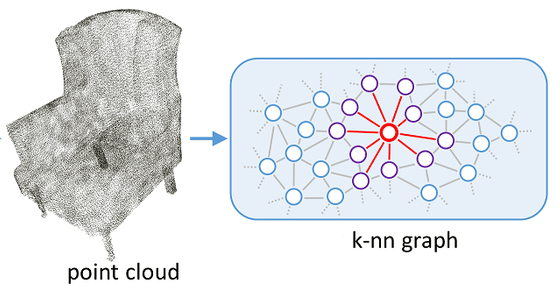
\includegraphics[width=\textwidth]{imagenes/chapter3/PatchSelection}
      \end{center}
      \caption{Extracción de características del vecindario.}
    \end{figure}
    \end{columns}
\end{frame}

\note{
Antes de probar directamente con modelos de DL, experimentamos con un método de 
ML. Dicho método está basado en la extracción de características de escena y entrenamiento de un 
modelo de vectores soporte para la regresión. 
Zhang y sus colaboradores proponen utilizar características geométricas y de 
color. Para la primera, extraen la curvatura, 
anisotropía, linealidad , 
planaridad y esfericidad de los puntos. 
Estas características se pueden extraer del vecindario 
de un punto por medio de la matriz de covarianza y los valores singulares 
de los K-vecinos más cercanos. Se calcularan para todos los puntos. 
Utilizaremos los valores medios, desviación y la entropía de estas características.
Además, calcularemos sus distancias a las distribuciones gaussiana y gamma, 
dado que se observó que la distribución de estas se veía afectada por la intensidad 
de las distorsiones. 
Las características lumínicas la descartamos, 
ya que información de textura o color no existe en los volúmenes
médicos habituales. 

}

\begin{frame}
  \frametitle{Modelo VQA-PC\footnote[frame]{\cite{VQA-PC}}}
  \begin{columns}
    \column{0.5\textwidth}
    \begin{enumerate}
      \item \textbf{Extracción automática} de características.
      \item Extracción \textbf{espacial y temporal} de las reconstrucciones.
        \begin{itemize}
          \item Espacial por fotogramas estáticos de \textbf{distintas perspectivas}.
          \item Temporal por tratar la \textbf{nube como video}.
        \end{itemize}
      \item Es como un \textbf{meta-modelo} de aprendizaje profundo. 
    \end{enumerate}
    \column{0.5\textwidth}
    \begin{figure}
      \begin{center}
        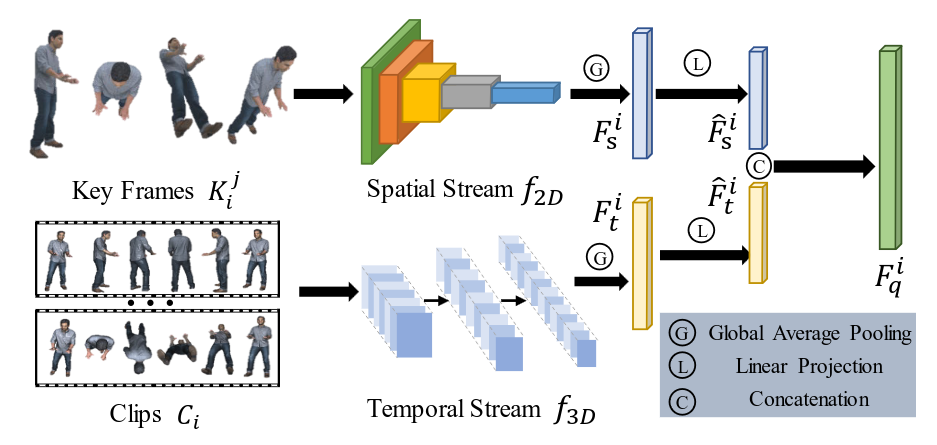
\includegraphics[width=\textwidth]{imagenes/chapter3/PipelineCompleto}
      \end{center}
      \caption{Estructura del modelo VQA-PC\footnotemark[10]}
    \end{figure}
  \end{columns}
\end{frame}

\note{
Por otro lado, en DL se propone un modelo de estimación de calidad de nubes 
de puntos utilizando proyecciones 2D, pero desde múltiples perspectivas. 
Zhang y sus colaboradores argumentan que los métodos anteriores de proyección 
se basan en la hipótesis de que los humanos percibimos la calidad de modelos 
3D desde una perspectiva estática, cosa que no 
es cierta en la práctica dado que los objetos 3D permiten operaciones geométricas 
de rotación y escalado.
Y por ello, siguiendo la motivación de que las deformaciones geométricas 
no deseados se presentan de forma abrupta según la perspectiva, proponen 
unificar la percepción estática con la dinámica tratando 
a las nubes de puntos como vídeos del objeto 3D rotando.
}

\subsection{Entorno}
\begin{frame}
  \frametitle{Tecnologías utilizadas}
  \begin{table}[htp]
    \vspace{-.5cm}
      \begin{tabular}{cccc}
        \begin{minipage}{.2\textwidth}
          
\includegraphics[width=\textwidth]{imagenes/chapter3/Python}
        \end{minipage} 
                                  & 
        \begin{minipage}{.2\textwidth}
          
\includegraphics[width=.9\textwidth]{imagenes/chapter3/FastAI}
        \end{minipage} 
                                  & 
        \begin{minipage}{.2\textwidth}
          
\includegraphics[width=\textwidth]{imagenes/chapter3/Pytorch}
        \end{minipage} 
                                  &
        \begin{minipage}{.2\textwidth}
          
\includegraphics[width=.9\textwidth]{imagenes/chapter3/Open3D}
        \end{minipage} 
                                  \\
        \begin{minipage}{.2\textwidth}
          
\includegraphics[width=\textwidth]{imagenes/chapter3/Numpy}
        \end{minipage} 
                                                        & 
        \begin{minipage}{.2\textwidth}
          
\includegraphics[width=.9\textwidth]{imagenes/chapter3/Scikit}
        \end{minipage} 
                                                        & 
        \begin{minipage}{.2\textwidth}
          
\includegraphics[width=.9\textwidth]{imagenes/chapter3/Polars}
        \end{minipage} 
        &
                                                        \\
                                                        & 
        \begin{minipage}{.2\textwidth}
          
\includegraphics[width=.9\textwidth]{imagenes/chapter3/Nvidia}
        \end{minipage} 
                                                        & 
        \begin{minipage}{.2\textwidth}
          
\includegraphics[width=.9\textwidth]{imagenes/chapter3/Colab}
        \end{minipage} 
                                                        &
                                                        \\
      \end{tabular}
  \end{table}
\end{frame}

\note{
Para el desarrollo y ejecución de los modelos fue necesario el uso de
la librería de DL Pytorch junto con las librerías CUDA para poder ejecutar 
los modelos en las tarjetas gráficas de NVIDIA. Para los cálculos numéricos y 
el manejo de datos se utilizaron Numpy y Polars. Teniendo en cuenta que para el
cálculo de las métricas hemos utilizado la librería de scikit-learn.
Para la visualización y fácil manipulación de las nubes de puntos se hizo uso 
de la librería de Open3D y Pyntcloud.
}

\section{Experimentación}
\subsection{Protocolo de validación}
\begin{frame}
  \frametitle{Protocolo de validación}
\begin{figure}[htp]
 \begin{center}
   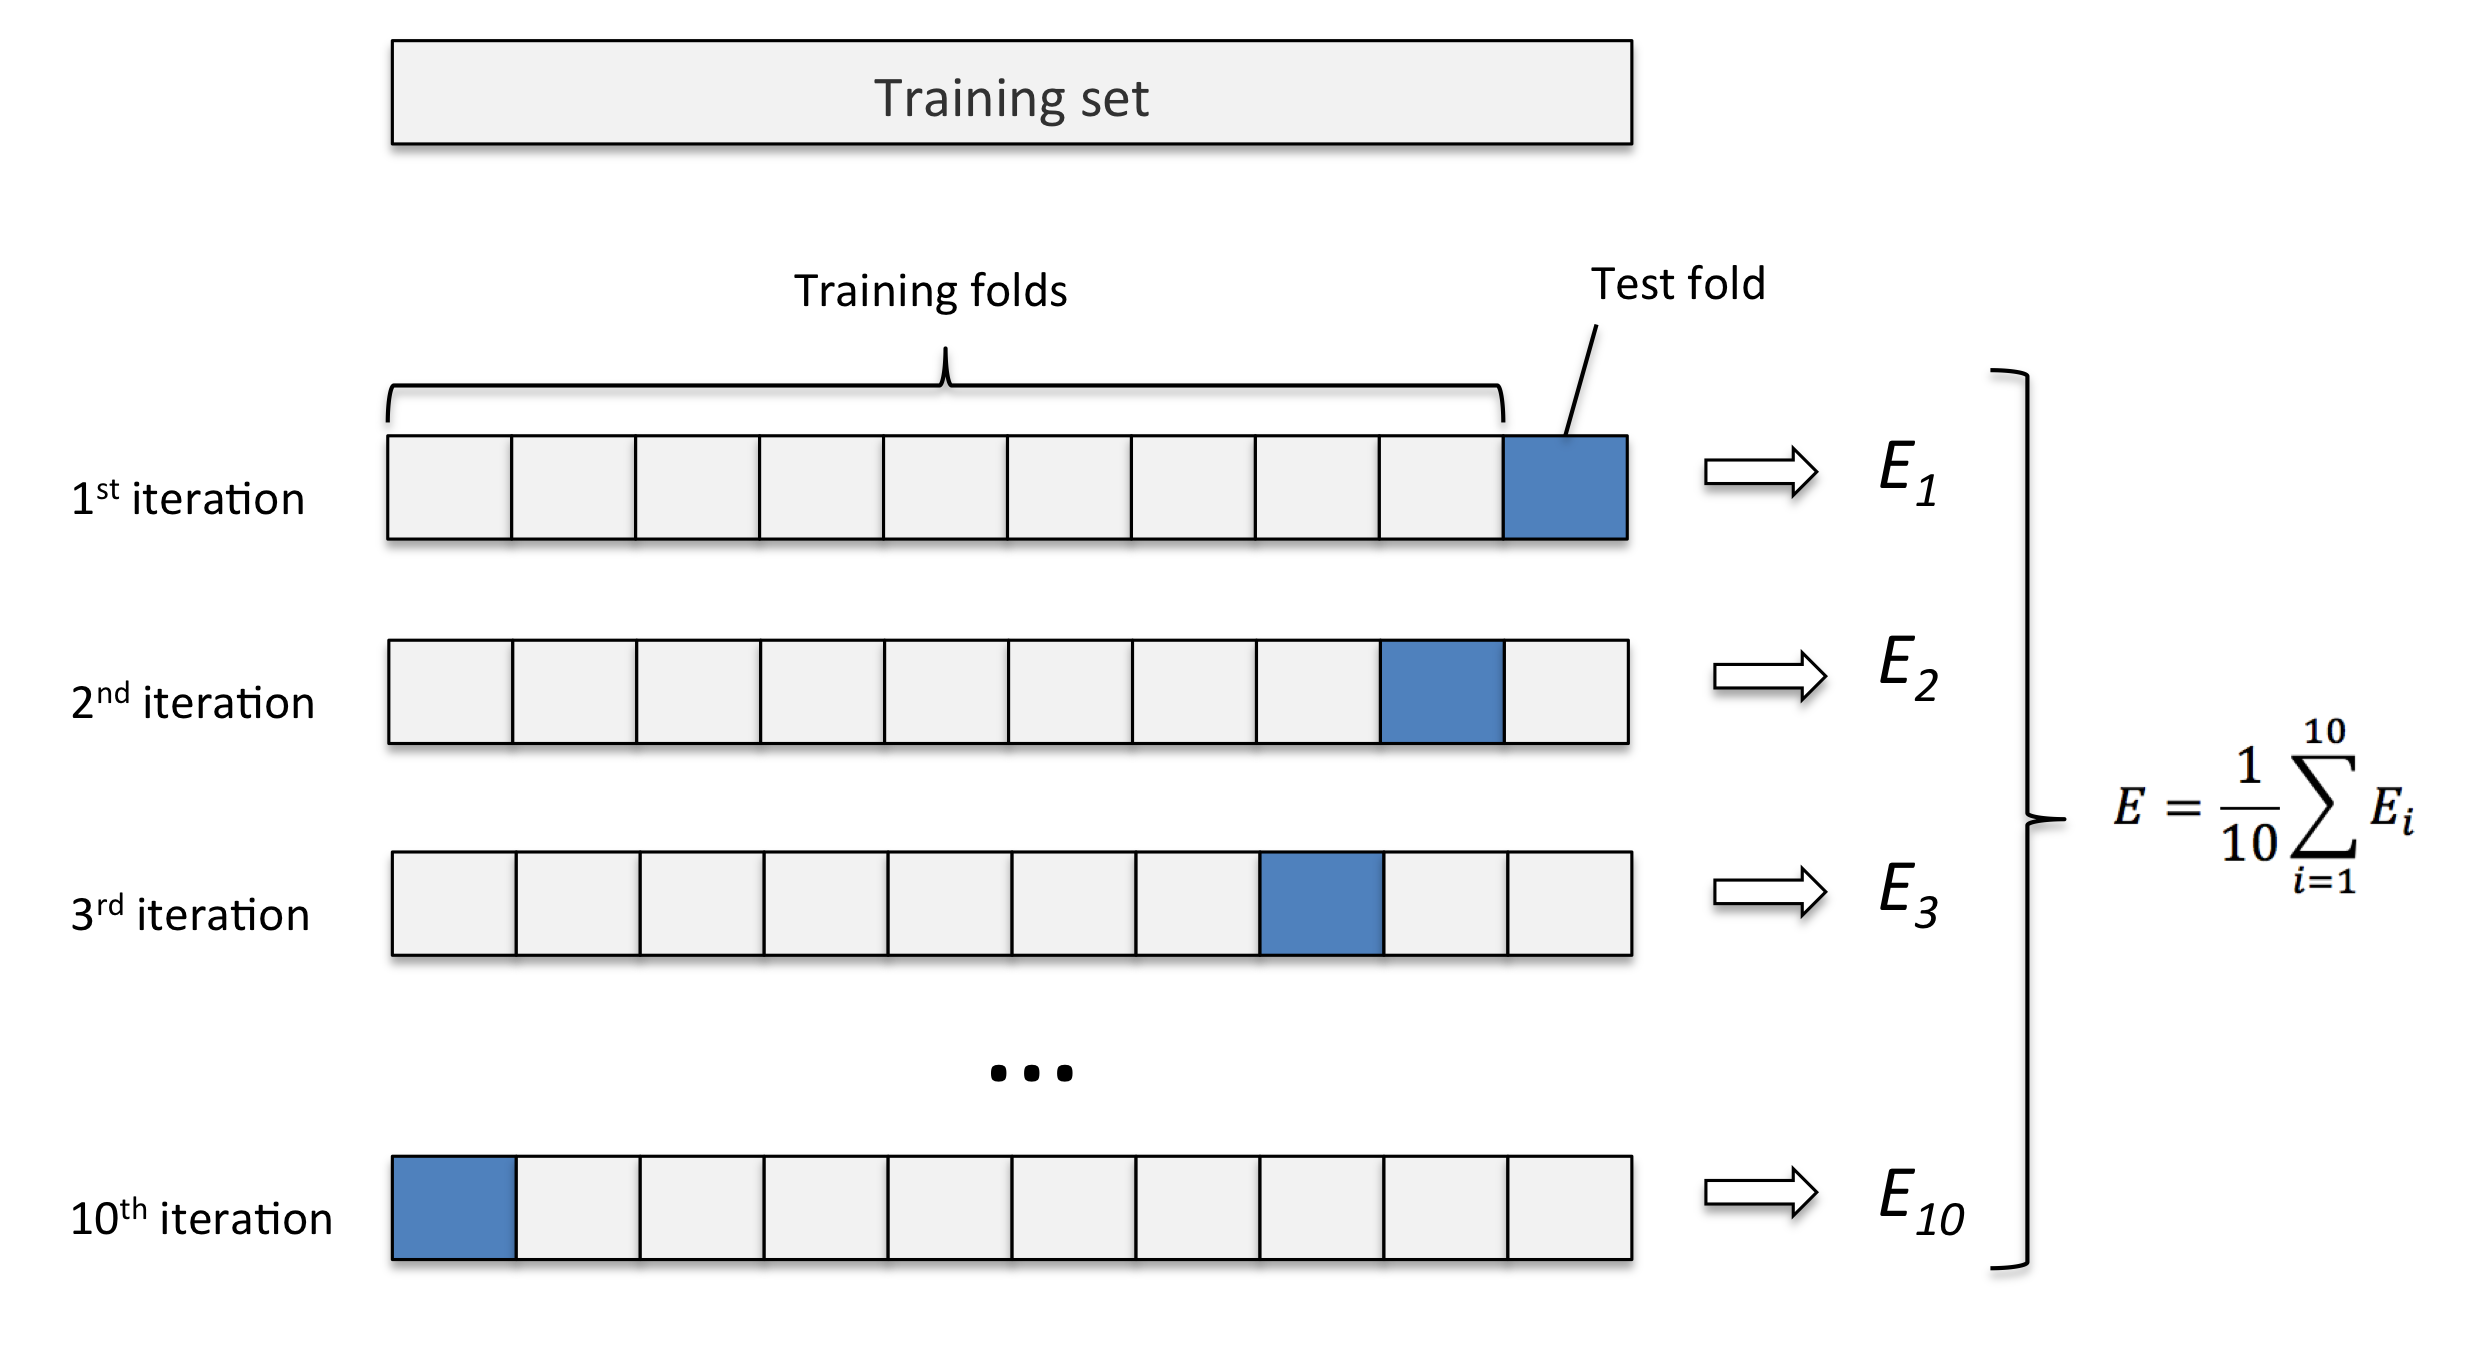
\includegraphics[width=.8\textwidth]{imagenes/chapter4/cross-validation}
 \end{center}
\end{figure}

\end{frame}

\subsection{Modelo NR3DQA}
\begin{frame}
  \frametitle{Modelo NR3DQA\footnotemark[11]}
\begin{table}[htp]
  \small
  \begin{center}
    \begin{tabular}[c]{|c|c|c|c|c|}
      \hline
      \rowcolor[HTML]{FFC702}
      \textbf{Dataset} & \textbf{PLCC} & \textbf{SROCC} & \textbf{KROCC} \\ 
      \hline
      SJTU & \textbf{0.810325} & \textbf{0.777403} & \textbf{0.608302} \\ 
      \hline 
      WPC & 0.637953 & 0.634853 & 0.463578 \\
      \hline
    \end{tabular}
  \end{center}
  \caption[Resultados de prueba preliminar con SVM.]{Replicando experimentos de Zhang et al\footnotemark[11].}
  \label{tab:PlainNR3DQA}
\end{table}
\begin{table}[htp]
  \small
  \begin{center}
    \hspace{-.5cm}
    \begin{tabular}[c]{|c|c|c|c|c|}
      \hline
      \rowcolor[HTML]{FFC702}
      \multicolumn{1}{|c|}{\textbf{Etiqueta Sintética}} & 
      \multicolumn{1}{|c|}{\textbf{Modelo}} & 
      \multicolumn{1}{|c|}{\textbf{Escalado}} & 
      \multicolumn{1}{|c|}{\textbf{PLCC}} &
      \multicolumn{1}{|c|}{\textbf{SROCC}} \\
      \hline
      Valor de la métrica & SVM & RobustScaler & 0.2017 & 0.1776 \\
      \hline
      Valor normalizado & KNNRegressor & RobustScaler & 0.2671 & 0.1882  \\
      \hline
      Valor en escala 0-5 & DecisionTree & StandardScaler & \textbf{0.309176} & \textbf{0.196713} \\
      \hline
    \end{tabular}
  \end{center}
  \caption[Resultados de prueba preliminar con NR3DQA.]{
    Resultados de prueba preliminar con NR3DQA\footnotemark[11]. 
  }
  \label{tab:MedicalNR3DQA}
\end{table}
    \footcitetext{NR3DQA}

\end{frame}

\begin{frame}
  \frametitle{Modificaciones}
  \begin{columns}
    \column{0.5\textwidth}
    \begin{itemize}
      \item Weinmann et al\footnotemark ~estudiaron los procesos de: 
        \begin{itemize}
          \item Segmentación.
          \item Detección.
          \item Clasificación.
        \end{itemize}
      \item Justifican la importancia de:  
        \begin{itemize}
          \item Omnivarianza.
          \item Entropía de los valores singulares.
          \item Verticalidad del vecindario.
        \end{itemize}
    \end{itemize}
    \column{0.5\textwidth}
  \begin{table}[htp]
    \small
    \begin{center}
      \begin{tabular}[c]{|c|c|c|c|c|}
        \hline
        \rowcolor[HTML]{FFC702}
        \textbf{Dataset} & \textbf{PLCC} & \textbf{SROCC} & \textbf{KROCC} \\ 
        \hline
        SJTU & \textbf{0.853709} & \textbf{0.820057} & \textbf{0.649406} \\ 
        \hline 
        WPC & 0.642356 & 0.62917 & 0.455562 \\
        \hline 
        Nuestro & 0.344601 &  0.170793 & -- \\
        \hline
      \end{tabular}
    \end{center}
    \caption[Resultado de mejoras sobre el método SVM]{Resultado de mejoras sobre el método SVM.}
    \label{tab:ImprovNR3DQA}
  \end{table}
\end{columns}
\footcitetext{3DNSSMetrics}
\end{frame}


\subsection{Modelo VQA-PC}
\begin{frame}
  \frametitle{Hiperparámetros del modelo VQA-PC\footnotemark[12]}
    \begin{columns} 
      \column{0.5\textwidth}
\bgroup
\begin{table}[htp]
  \vspace{-.4cm}
  \scriptsize
  \begin{center}
    % \[\setcellgapes{5pt}\makegapedcells % <--- for vertical space around cells contents
    \begin{tabular}[b]{|c|c|}
      \hline
      \rowcolor[HTML]{FFC702}
      \multicolumn{1}{|c|}{\textbf{Salida}}  &
      \multicolumn{1}{c|}{\textbf{Estructura}} \\
      \hline
      $112\times112$ & $7\times7,\; 64$, stride 2 \\ 
      \hline 
      \multirow{2}{*}{$56\times56$} & $3\times3$ max pool, stride 2 \\ 
      \cline{2-2}
      & $\begin{bmatrix}1\times1,\; 64 \\ 3\times3,\; 64 \\ 1\times1,\; 256 \end{bmatrix}\times 3$ \\ 
      \hline
      $28\times28$ & $\begin{bmatrix}1\times1,\; 128 \\ 3\times3,\; 128 \\ 1\times1,\; 512 \end{bmatrix}  \times 3 $\\ 
      \hline
      $14\times14$ & $\begin{bmatrix}1\times1,\; 256 \\ 3\times3,\; 256 \\ 1\times1,\; 1024 \end{bmatrix} \times 3$ \\ 
      \hline
      $7\times7$   & $\begin{bmatrix}1\times1,\; 512 \\ 3\times3,\; 512 \\ 1\times1,\; 2048 \end{bmatrix}  \times 3 $\\ 
      \hline
      $1\times1$   & average pool, 1000-d fc, softmax\\ 
      \hline
      \end{tabular}
    % \]
  \end{center}
  \caption{Descripción de la arquitectura ResNet50.}
  \label{tab:ResNet50}
\end{table}
\egroup

      \column{0.5\textwidth}
  \begin{table}[htp]
    \small
    \begin{center}
      \begin{tabular}[c]{|c|c|}
        \hline
        \rowcolor[HTML]{FFC702}
        \textbf{Hiperparámetro} & \textbf{Valor} \\ 
        \hline 
        Tasa de aprendizaje &  0.0004 \\ 
        \hline 
        Tamaño de batches & 32 \\ 
        \hline 
        Tasa de decadencia & 0.9 \\ 
        \hline 
        Frecuencia de decadencia & 10 \\ 
        \hline 
        Épocas & 30 \\ 
        \hline 
        K-fold & 9 \\ 
        \hline 
      \end{tabular}
    \end{center}
    \caption[Hiperparámetros empleados en la experimentación preliminar.]{
      Hiperparámetros empleados en la experimentación preliminar\footnotemark[12]
    }
      \vspace{-.6cm}
    \label{tab:HiperSJTU}
  \end{table}
  \footcitetext{VQA-PC}
    \end{columns}
\end{frame}

\begin{frame}
  \frametitle{Experimentos preliminares VQA-PC}
\begin{table}[htp]
  \small
  \begin{center}
    \begin{tabular}[c]{|c|c|c|}
      \hline
      \rowcolor[HTML]{FFC702}
      \textbf{Kfold} & \textbf{MSE} & \textbf{SROCC} \\ 
      \hline 
      0 & 13.9222 & 0.8995 \\
      \hline 
      1 & 418120.5625 & 0.8547 \\ 
      \hline 
      2 & 10.9271 & 0.9081 \\
      \hline 
      3 & 19.8226 & 0.9295 \\ 
      \hline 
      4 & 443.6077 & 0.8700 \\ 
      \hline 
      5 & 28.3165 & 0.9544 \\ 
      \hline 
      6 & 292.239 & 0.7675 \\ 
      \hline 
      7 & 329.0685 & 0.8833 \\ 
      \hline 
      8 & 357.0455 & 0.8647 \\ 
      \hline
      \textbf{\cellcolor[HTML]{FFC702}Promedio} & \textbf{46623.94} & \textbf{0.8813} \\ 
      \hline
    \end{tabular}
  \end{center}
  \caption[Resultados de experimento preliminar.]{
    Resultados de experimento preliminar. 
  }
  \label{tab:PreTestResults}
\end{table}
\end{frame}

\begin{frame}
  \frametitle{Curvas de aprendizaje VQA-PC}
  \vspace{-.5cm}
\begin{figure}[htp]
  \centering
    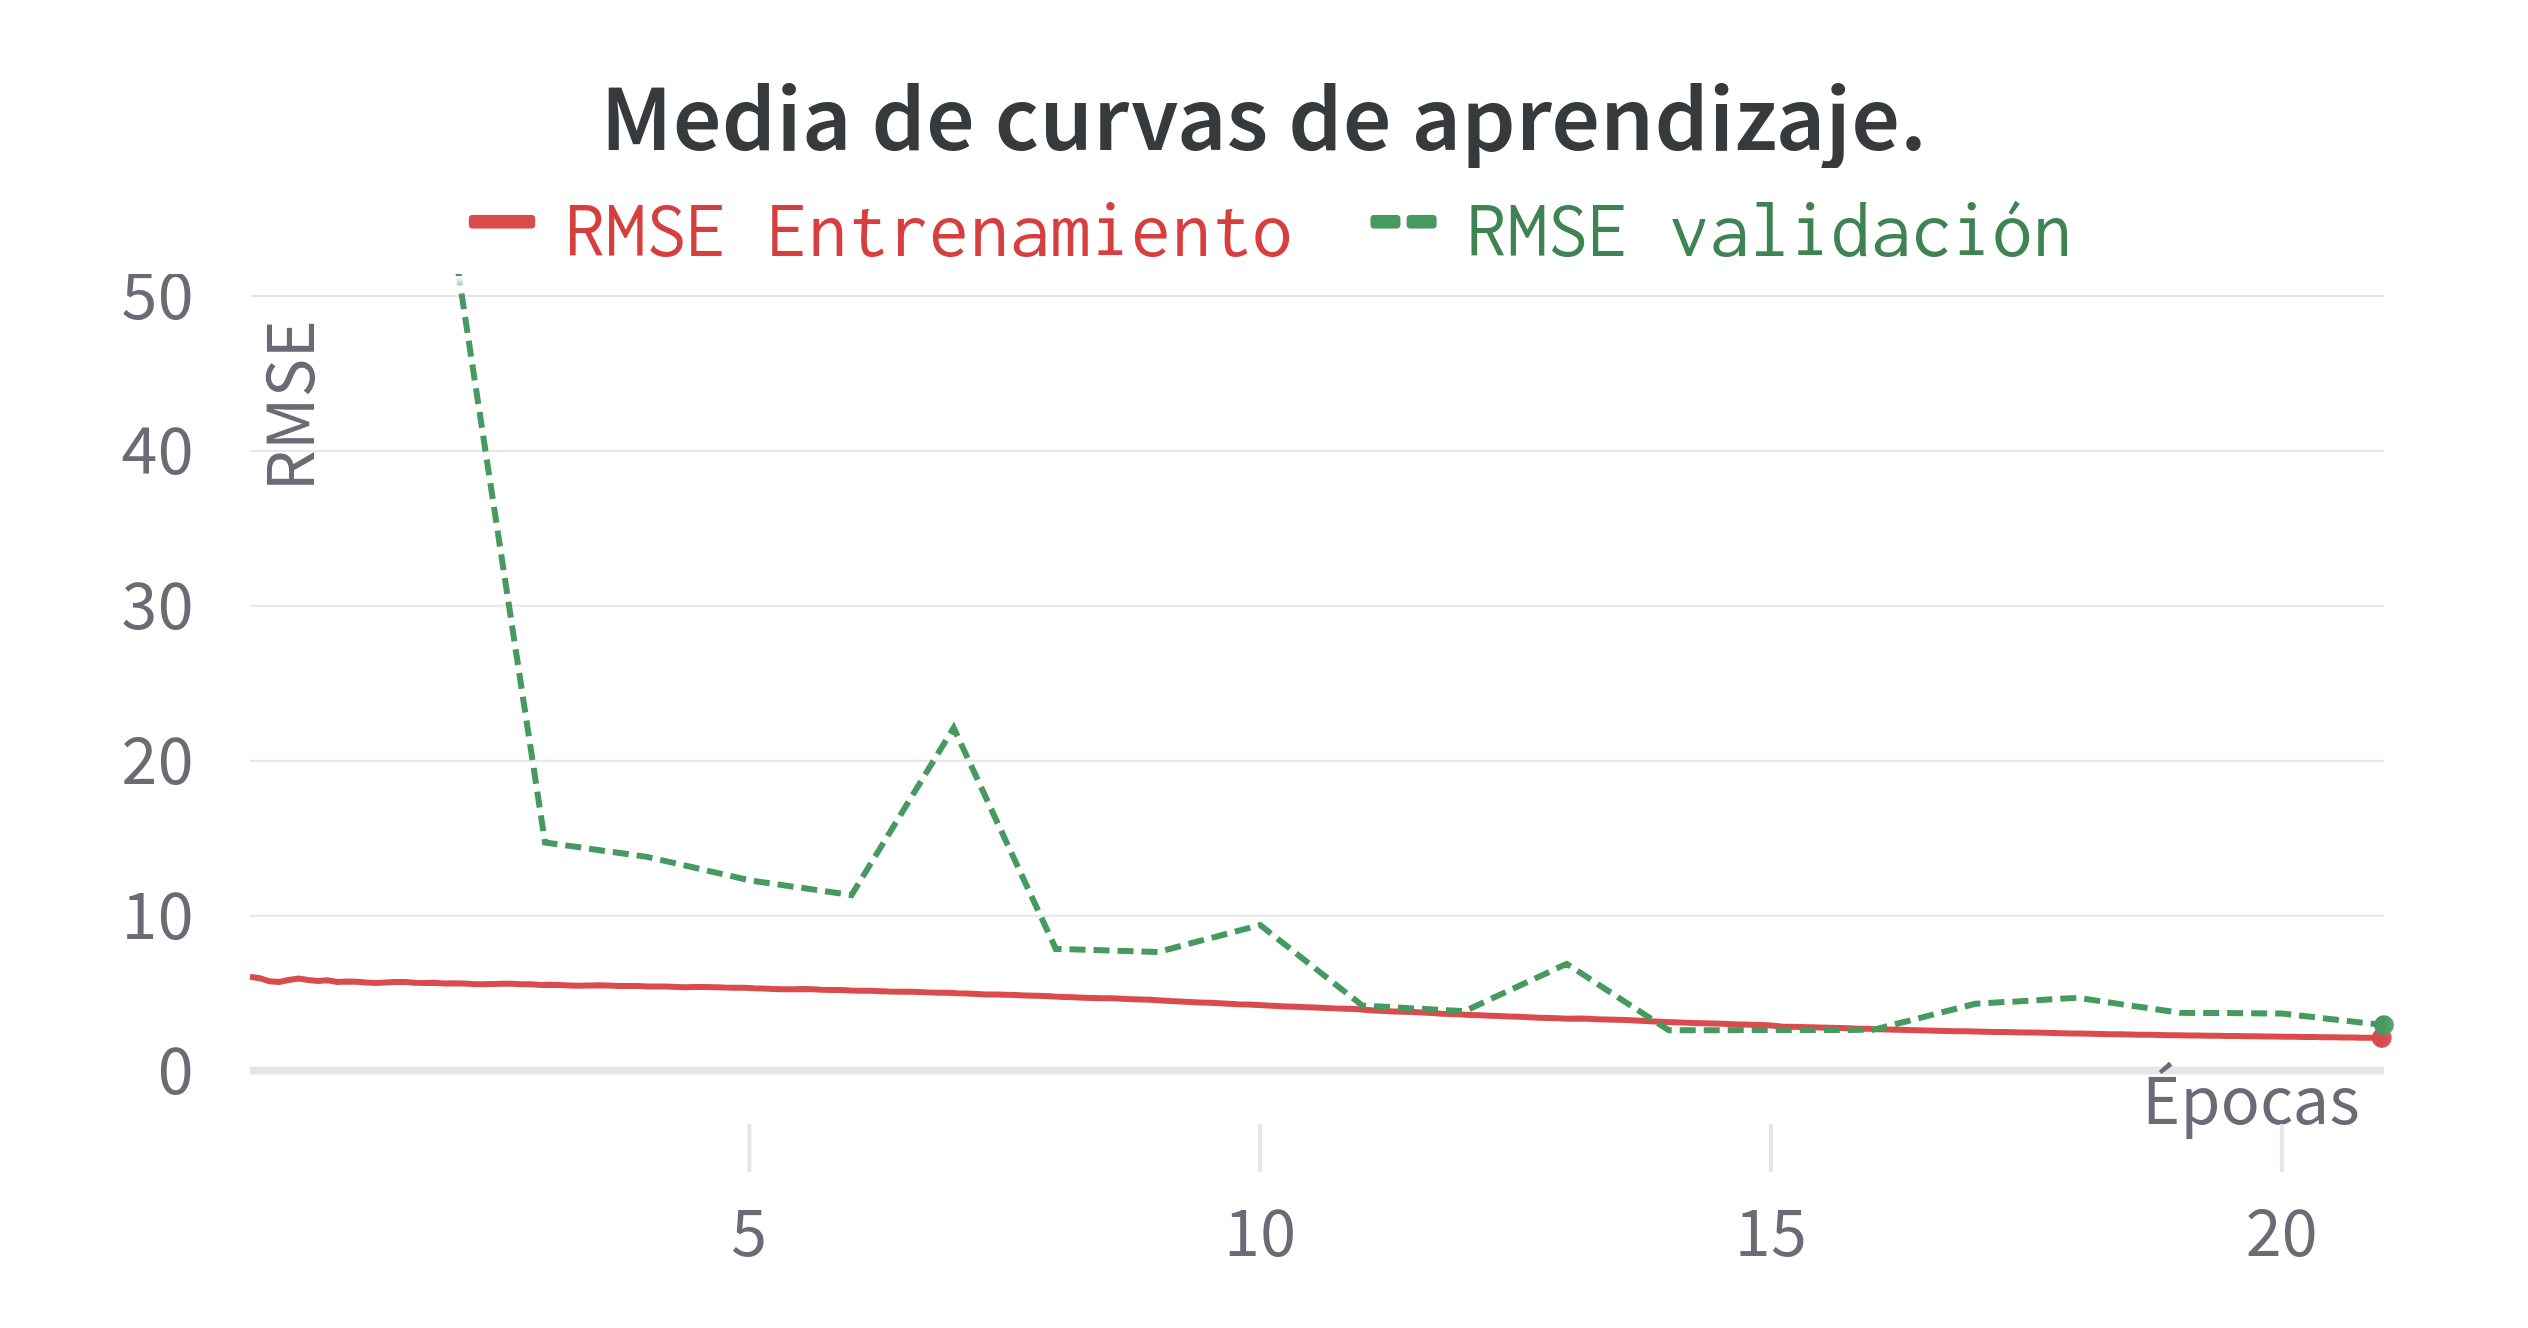
\includegraphics[width=.75\textwidth]{imagenes/chapter4/PreTestCurves.png}
  \caption[Curvas de aprendizaje del test preliminar.]{
    Curvas de aprendizaje del test preliminar. 
  } 
\label{fig:PreTestCurves}
\end{figure}
\end{frame}

\begin{frame}
  \frametitle{Modificaciones}
  \begin{enumerate}
    \item Abouelaziz et al\footnotemark~ experimentaron \alert{distintos métodos de fusión de características}.
      \begin{itemize}
        \item Fusión por \textbf{concatenación} (F0).
        \item Fusión por \textbf{multiplicación} (F1). 
        \item Fusión por \textbf{convolución 1x1} (F2).
        \item Fusión por \textbf{\emph{compact multi-linear pooling}} (F3).
      \end{itemize}
    \item Experimentamos con todas ellas.
    \item Experimentamos con \textbf{etiquetas normalizadas o no}.
    \item En vez de recortar una selección local, \textbf{reescalar la imagen entera}.
  \end{enumerate}
  \footcitetext{EnsemblePCQA}
\end{frame}

\begin{frame}
  \frametitle{Experimentos finales VQA-PC}
\begin{table}[htp]
  \small
  \centering
\begin{tabular}{|c|cccc|}
\hline
\rowcolor[HTML]{FFC702}
                       & \multicolumn{4}{c|}{\textbf{Valor medio SROCC}}                                                                                                    \\ \hline
\rowcolor[HTML]{FFC702}
\textbf{Modelo}        & \multicolumn{1}{c|}{\textbf{Estándar}} & \multicolumn{1}{c|}{\textbf{Normalizado}} & \multicolumn{1}{c|}{\textbf{Reescalado}} & \textbf{Ambos}  \\ \hline
\textbf{VQA-PC (SJTU)} & \multicolumn{1}{c|}{0.7094}            & \multicolumn{1}{c|}{\textbf{0.6235}}      & \multicolumn{1}{c|}{\textbf{0.8425}}    & 0.7126          \\ \hline
\textbf{VQA-PC F1}     & \multicolumn{1}{c|}{\textbf{0.7305}}   & \multicolumn{1}{c|}{0.6140}               & \multicolumn{1}{c|}{0.8164}             & 0.7291          \\ \hline
\textbf{VQA-PC F2}     & \multicolumn{1}{c|}{0.6816}            & \multicolumn{1}{c|}{0.5770}               & \multicolumn{1}{c|}{0.8057}             & \textbf{0.7324} \\ \hline
\textbf{VQA-PC F3}     & \multicolumn{1}{c|}{0.7080}            & \multicolumn{1}{c|}{0.5671}      & \multicolumn{1}{c|}{0.7482}             & 0.7006          \\ \hline
\end{tabular}
\caption[Valor medio sobre imágenes médicas.]{Tabla de resultados iniciales sobre imágenes médicas.}
\label{tab:SroccMedRes}
\end{table}
\end{frame}

\begin{frame}
  \frametitle{Experimentos finales VQA-PC}
\begin{table}[htp]
  \small
  \centering
\begin{tabular}{|c|cccc|}
\hline
\rowcolor[HTML]{FFC702}
                       & \multicolumn{4}{c|}{\textbf{Mediana SROCC}}                                                                                                          \\ \hline
\rowcolor[HTML]{FFC702}
\textbf{Modelo}        & \multicolumn{1}{c|}{\textbf{Estándar}} & \multicolumn{1}{c|}{\textbf{Normalizado}} & \multicolumn{1}{c|}{\textbf{Reescalado}} & \textbf{Ambos}  \\ \hline
\textbf{VQA-PC (SJTU)} & \multicolumn{1}{c|}{\textbf{0.7400}}   & \multicolumn{1}{c|}{\textbf{0.7510}}      & \multicolumn{1}{c|}{0.8417}             & 0.7434          \\ \hline
\textbf{VQA-PC F1}     & \multicolumn{1}{c|}{0.7022}            & \multicolumn{1}{c|}{0.6331}               & \multicolumn{1}{c|}{\textbf{0.8636}}    & \textbf{0.7849} \\ \hline
\textbf{VQA-PC F2}     & \multicolumn{1}{c|}{0.6350}            & \multicolumn{1}{c|}{0.5955}               & \multicolumn{1}{c|}{0.8538}             & 0.7165          \\ \hline
\textbf{VQA-PC F3}     & \multicolumn{1}{c|}{0.7118}            & \multicolumn{1}{c|}{0.5179}               & \multicolumn{1}{c|}{0.7518}             & 0.7334          \\ \hline
\end{tabular}
\caption[Mediana de los valores sobre imágenes médicas.]{
  Mediana de los valores obtenidos. Se observa una mejora significativa para 
  los métodos F1 y F2. También es evidente la estabilidad del modelo pre-entrenado sobre SJTU. 
}
\label{tab:PercentileMed}
\end{table}
\end{frame}

\begin{frame}
  \frametitle{Resultados Finales}
\begin{table}[H]
  \small 
  \centering
\begin{tabular}{|c|c|c|c|}
\hline
\rowcolor[HTML]{FFC702}
                       & \multicolumn{3}{c|}{\textbf{SROCC}}                                                                                                          \\ \hline
\rowcolor[HTML]{FFC702}
\textbf{Modelo}    & \textbf{Media} & \textbf{Desviación} & \textbf{Mediana} \\ \hline
\textbf{VQA-PC F0} & 0.8325           & 0.2017              & 0.9140           \\ \hline
\textbf{VQA-PC F1} & 0.8242           & 0.2025              & 0.9095           \\ \hline
\textbf{VQA-PC F2} & \textbf{0.8757}  & \textbf{0.1468}     & \textbf{0.9347}  \\ \hline
\textbf{VQA-PC F3} & 0.8071           & 0.1811              & 0.8692           \\ \hline
\end{tabular}
\caption[Resultados en imágenes médicas reescaladas entrenando en LS-PCQA.]{
  Resultados en imágenes médicas reescaladas con modelos pre-entrenados 
  sobre el conjunto de datos LS-PCQA\footnotemark[10]. 
}\label{tab:LS-PCQA-FN}
\end{table}
\footcitetext{ResSCNN}
\end{frame}



\section{Conclusiones y trabajos futuros}
\subsection{Conclusiones}

\begin{frame}
  \frametitle{Conclusiones}
  \begin{enumerate}
    \item \textbf{Primer método} que estima la calidad de reconstrucciones biomédicas 3D.
    \item Se logra generar un \textbf{conjunto de datos médicos sintéticos } para estimación de calidad.
    \item \textbf{Se justifica} el uso de modelos de \textbf{aprendizaje profundo} \alert{experimentalmente}.
    \item Pese a ser un estudio preliminar, obtenemos una \textbf{alta correlación (88\%)}. Indicador 
      de lo prometedora que es esta línea de investigación.
  \end{enumerate}
\end{frame}

\begin{frame}
    \frametitle{Conclusiones}
\begin{figure}
  \vspace{-.5cm}
  \hspace{-.2cm}\subfloat[Submuestreo al 10\%]{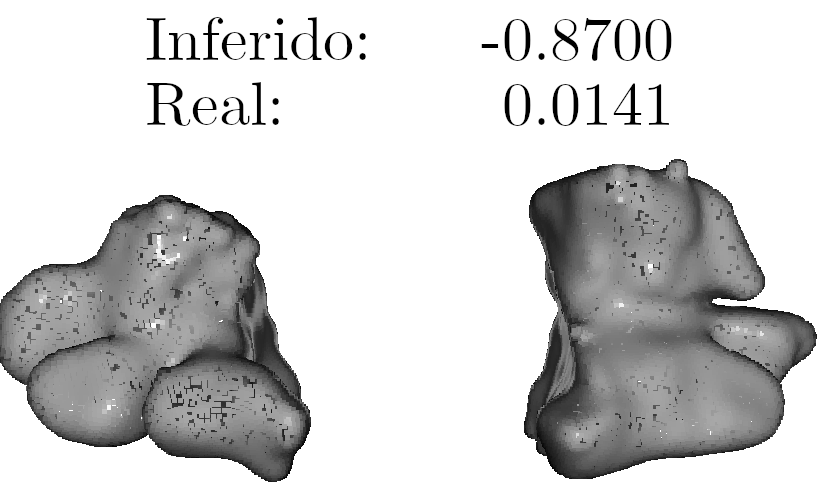
\includegraphics[width=.3\textwidth]{imagenes/chapter5/Maxiliar100014_7.png}}\hspace{.2cm}
  \subfloat[Submuestreo al 30\%]{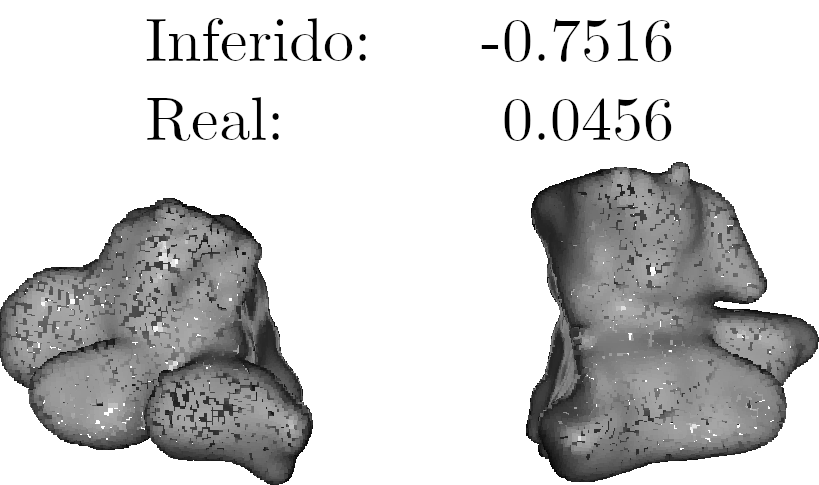
\includegraphics[width=.3\textwidth]{imagenes/chapter5/Maxiliar100014_9.png}}\hspace{.2cm}
  \subfloat[Submuestreo al 60\%]{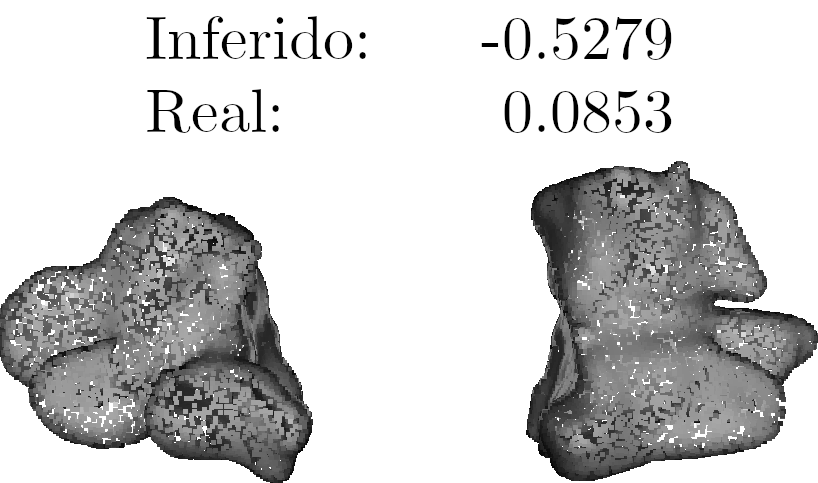
\includegraphics[width=.3\textwidth]{imagenes/chapter5/Maxiliar100014_11.png}}
  \caption{Ejemplo de correspondencia de pendiente entre valores inferidos (sin normalizar) y 
  los valores reales de las etiquetas.} 
  \label{fig:Cualitativos}
\end{figure}
\vspace{-.5cm}
\begin{enumerate}
  \item Se han completado satisfactoriamente los objetivos planteados.
  \item Se han abierto puertas a futuras investigaciones.
  \item \url{https://github.com/CodeBoy-source/TFG_NRPCQA} 
\end{enumerate}
\end{frame}

\begin{frame}
  \frametitle{Trabajos futuros}
  \begin{enumerate}
    \item Rehacer el experimento con \textbf{etiquetas generadas manualmente}. 
    \item \textbf{Para mejorar el meta-modelo}, se podria \alert{permitir la adaptación} del modelo de extracción de características \textbf{temporales}.
    \item Simular distorsiones sobre \textbf{imágenes 2D} para obtener datos más \textbf{realistas}.
    \item Explorar \alert{otros métodos} de la literatura. 
  \end{enumerate}
\end{frame}




\end{document} 

